The basis functions that go hand in hand with the open Newton--Cotes rule are
the following piecewise linear functions. For $i = 0$ and $j = 0$,
\[
  \e_{00}(\x) = 1.
\]
For $i > 0$ and $j = 0$ (close to the left endpoint),
\[
  \e_{i0}(\x) = \begin{cases}
    2 - \left( \n_i + 1 \right) \x, & \text{if } \x < \frac{2}{\n_i + 1}, \\
    0, & \text{otherwise}.
  \end{cases}
\]
For $i > 0$ and $j = \n_i - 1$ (close to the right endpoint),
\[
  \e_{i(\n_i - 1)}(\x) = \begin{cases}
    \left( \n_i + 1 \right) \x - \n_i + 1, & \text{if } \x > \frac{\n_i - 1}{\n_i + 1}, \\
    0, & \text{otherwise}.
  \end{cases}
\]
In other cases,
\[
  \e_{ij}(\x) = \begin{cases}
    1 - \left( \n_i + 1 \right)|\x - \x_{ij}|, & \text{if } |\x - \x_{ij}| < \frac{1}{\n_i + 1}, \\
    0, & \text{otherwise}.
  \end{cases}
\]
The basis functions corresponding to the first three levels of one-dimensional
interpolation are depicted in \fref{basis}. Note that $\e_{11}$, $\e_{21}$,
$\e_{23}$, and $\e_{25}$ are not depicted as they are not involved in the
hierarchical construction. In multiple dimensions, the basis functions are
formed as shown in \eref{basis-functions}.

\begin{figure}[t]
  \centering
  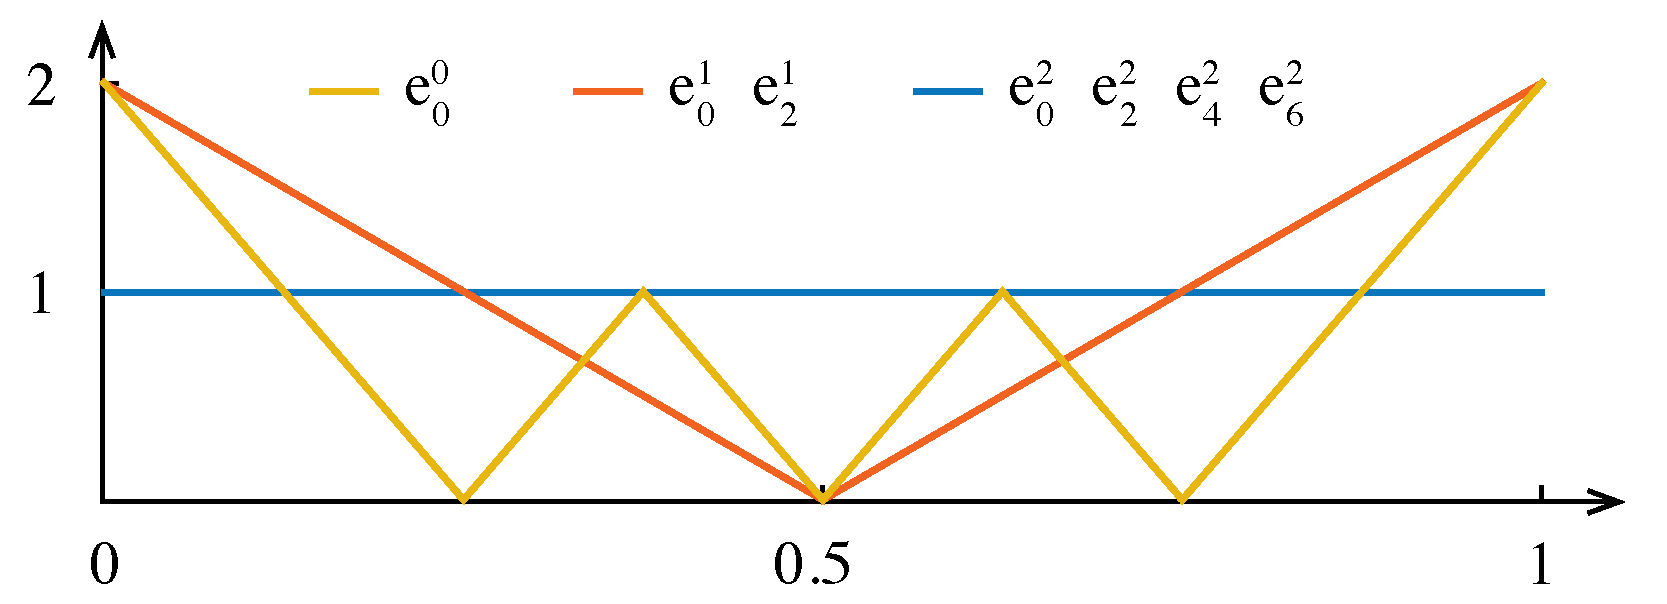
\includegraphics[width=1.0\columnwidth]{include/assets/figures/basis.pdf}
  \vspace{-1.5em}
  \caption{
    The first three levels of the basis described in \sref{basis}.
  }
  \flab{basis}
\end{figure}

Lastly, let us mention the volumes (integrals over the whole domain) of the
basis functions denoted by $\w_{ij}$; they will be needed in the future. Namely,
$\w_{00} = 1$ and, for $i > 0$,
\begin{equation} \elab{volume}
  \w_{ij} = \int_0^1 \e_{ij}(\x) \, \d\x = \begin{cases}
    \frac{2}{\n_i + 1}, & \text{if } j \in \{ 0, \n_i - 1 \}, \\
    \frac{1}{\n_i + 1}, & \text{otherwise}.
  \end{cases}
\end{equation}
In multiple dimensions, the volumes are products of the one-dimensional
components, analogous to \eref{basis-function}.

\begin{remark}
Instead of piecewise linear functions, one can also utilize locally supported
polynomials of higher orders \cite{jakeman2012}. However, we did not observe
much improvement and, therefore, do not discuss this alternative in the paper.
\end{remark}
